\documentclass[12pt,a4paper]{article}

% =================================================
% LANGUE ET TYPOGRAPHIE
% =================================================
\usepackage[T1]{fontenc}
\usepackage[utf8]{inputenc}
\usepackage[french]{babel}
\usepackage{lmodern}
\usepackage{microtype}

% =================================================
% MISE EN PAGE
% =================================================
\usepackage[
    a4paper,
    top=2.7cm,
    bottom=2.5cm,
    left=2.7cm,
    right=2.7cm,
    headheight=16pt
]{geometry}

\usepackage{setspace}
\setstretch{1.15}
\setlength{\parindent}{0pt}
\setlength{\parskip}{6pt}

% =================================================
% COULEURS ET TITRES
% =================================================
\usepackage{xcolor}
\definecolor{bleufonce}{HTML}{17365D}
\definecolor{bleuclair}{HTML}{DCE6F1}
\definecolor{gris}{HTML}{313131}

\usepackage{titlesec}

\titleformat{\section}
  {\Large\bfseries\color{bleufonce}}
  {\thesection.}{0.7em}{}
  [\vspace{3pt}\color{bleuclair}\titlerule]

\titleformat{\subsection}
  {\large\bfseries\color{bleufonce}}
  {\thesubsection}{0.7em}{}

\titlespacing*{\section}{0pt}{24pt}{12pt}
\titlespacing*{\subsection}{0pt}{16pt}{8pt}

% =================================================
% IMAGES ET LIENS
% =================================================
\usepackage{graphicx}
\usepackage{float}
\usepackage{hyperref}
\usepackage{placeins}

\hypersetup{
    colorlinks=true,
    linkcolor=bleufonce,
    urlcolor=bleufonce,
    pdftitle={Rapport de mi-projet C++},
    pdfauthor={Raïan CHOUIREF et Dorian LEON FERNANDES}
}

% =================================================
% EN-TÊTES ET PIEDS DE PAGE
% =================================================
\usepackage{fancyhdr}

\pagestyle{fancy}
\fancyhf{}

\fancyhead[L]{\small\textcolor{gris}{Rapport de mi-projet C++}}
\fancyhead[R]{\small\textcolor{gris}{Modélisateur 3D}}

\fancyfoot[L]{\small\textcolor{gris}{Raïan CHOUIREF -- Dorian LEON FERNANDES}}
\fancyfoot[R]{\small\textcolor{gris}{Page \thepage}}

\renewcommand{\headrulewidth}{0.4pt}
\renewcommand{\footrulewidth}{0.4pt}

% =================================================
% SOMMAIRE
% =================================================
\usepackage{tocloft}

\renewcommand{\contentsname}{Sommaire}
\renewcommand{\cftsecfont}{\bfseries\color{bleufonce}}
\renewcommand{\cftsecpagefont}{\bfseries\color{bleufonce}}
\setlength{\cftbeforesecskip}{8pt}

% =================================================
% DOCUMENT
% =================================================
\begin{document}

% =================================================
% PAGE DE GARDE
% =================================================
\begin{titlepage}
    \thispagestyle{empty}

    \centering

    \vspace*{2cm}

    {\Large\textcolor{gris}{RAPPORT DE MI-PROJET}\par}

    \vspace{1.5cm}

    {\color{bleufonce}\rule{\textwidth}{1.5pt}\par}

    \vspace{0.7cm}

    {\Huge\bfseries Rapport C++\par}

    \vspace{0.5cm}

    {\Large\textcolor{gris}{Structures de données et affichage 3D}\par}

    \vspace{0.7cm}

    {\color{bleufonce}\rule{\textwidth}{1.5pt}\par}

    \vspace{2.5cm}

    {\large\textbf{Réalisé par}\par}

    \vspace{0.5cm}

    {\Large Raïan CHOUIREF\par}
    \vspace{0.2cm}
    {\Large Dorian LEON FERNANDES\par}

    \vfill

    {\large Année universitaire : 2026--2027\par}

    \vspace{0.5cm}

    {\large \today\par}

    \vspace{1cm}

\end{titlepage}

% =================================================
% SOMMAIRE
% =================================================
\pagenumbering{roman}

\tableofcontents

\newpage

% =================================================
% CONTENU DU RAPPORT
% =================================================
\pagenumbering{arabic}

\section{Introduction}

Ce projet consiste à développer un éditeur 3D capable de charger, afficher et manipuler des modèles 3D à partir de fichiers aux formats .PLY et .OBJ. 
L'objectif principal est de permettre à l'utilisateur d'interagir avec les modèles 3D de manière intuitive et efficace. 
Pour cela, nous devons mettre en place une structure de données adaptée pour représenter les maillages 3D, ainsi qu'un système d'affichage performant utilisant OpenGL. 
Les grandes étapes du projet incluent la conception de la structure de données Halfedge, le développement du chargeur de fichiers, l'implémentation du système d'affichage et la création d'une interface utilisateur.

\section{Problème}

Dans ce projet, nous sommes confrontés à la problématique de la manipulation et de l'affichage de modèles 3D à partir de fichiers aux formats .PLY et .OBJ. L'objectif principal est de développer un éditeur 3D capable de charger ces fichiers, d'afficher les modèles correspondants et de permettre à l'utilisateur d'interagir avec eux. 
Les objectifs spécifiques du projet incluent :
\begin{itemize}
    \item La mise en place d'une structure de données efficace pour représenter les maillages 3D, notamment en utilisant la structure Halfedge.
    \item Le développement d'un système d'affichage utilisant OpenGL pour rendre les modèles 3D de manière réaliste et performante.
    \item La création d'un chargeur de fichiers capable de lire les formats .PLY et .OBJ, d'extraire les informations géométriques et de les convertir en structures de données utilisables par le programme.
\end{itemize}

\newpage
\section{Contexte du projet}

Dans le cadre de la matière Computer Science, nous avons été amenés à réaliser un projet en C++ portant sur la programmation et la géométrie. L'objectif principal de ce projet était de développer un éditeur 3D capable de charger, afficher et manipuler des modèles 3D à partir de fichiers aux formats .PLY et .OBJ. 
Pour ce faire, nous avons utilisé plusieurs outils et bibliothèques, notamment OpenGL pour le rendu graphique, ainsi que des structures de données adaptées pour représenter les maillages 3D. 
Les contraintes du projet incluaient la gestion efficace des données géométriques, la mise en place d'une interface utilisateur intuitive et la compatibilité avec différents formats de fichiers 3D. Nous avons également dû nous assurer que notre éditeur 3D soit capable de gérer des modèles complexes tout en maintenant des performances optimales.

Pour le moment, nous avons réussi à implémenter les fonctionnalités de base, le chargement des fichiers .PLY et .OBJ, ainsi que l'affichage des modèles 3D. Cependant, il reste encore des améliorations à apporter, notamment en ce qui concerne l'optimisation des performances et l'ajout de fonctionnalités supplémentaires pour enrichir l'expérience utilisateur.

\newpage

\section{UML}

\begin{figure}[H]
    \centering
    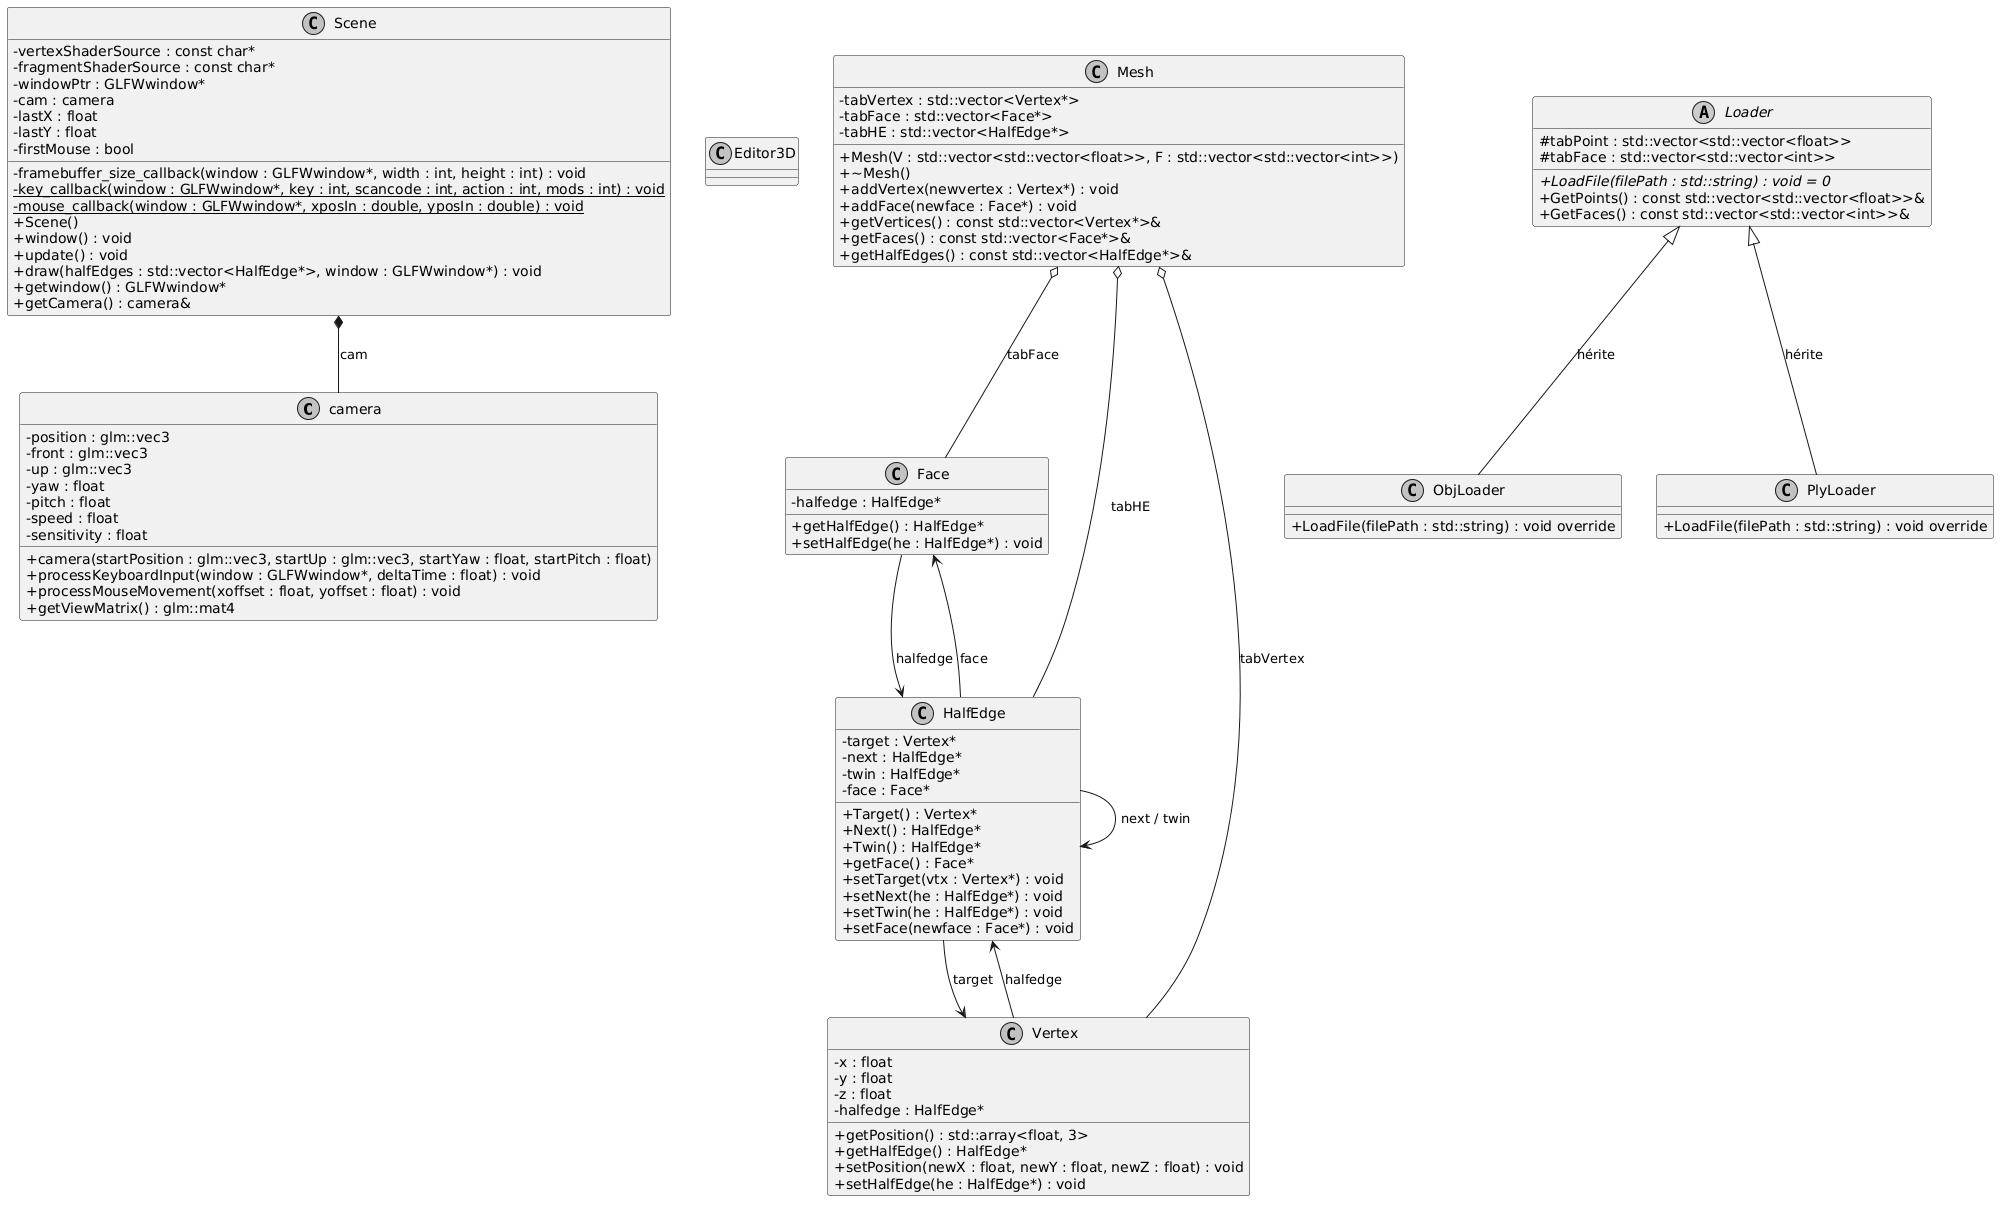
\includegraphics[width=1\textwidth]{uml.png}
    \caption{Diagramme UML du projet}
    \label{fig:uml}
\end{figure}

Nous avons utilisé un diagramme UML pour représenter les classes et leurs relations dans notre projet. Le diagramme montre les principales classes, leurs attributs et méthodes, ainsi que les associations entre elles. Cela nous a permis de mieux comprendre la structure du projet et de faciliter la communication entre les membres de l'équipe. 

Voici une explication des principales classes et de leurs relations :
\begin{itemize}
    \item La classe \texttt{Scene} représente la scène 3D et contient des objets tels que des maillages et des caméras. Elle est responsable de la gestion de l'affichage et de l'interaction avec les objets.
    \item La classe \texttt{Mesh} représente un maillage 3D et contient des informations sur les sommets, les faces et les arêtes. Elle est responsable de la gestion des données géométriques et de la génération des structures de données nécessaires pour l'affichage.
    \item La classe \texttt{Halfedge} représente une structure de données pour les maillages, permettant une navigation efficace entre les sommets, les arêtes et les faces. Elle est utilisée pour faciliter les opérations de modification et d'affichage des maillages.
\end{itemize}
 
\begin{figure}[H]
    \centering
    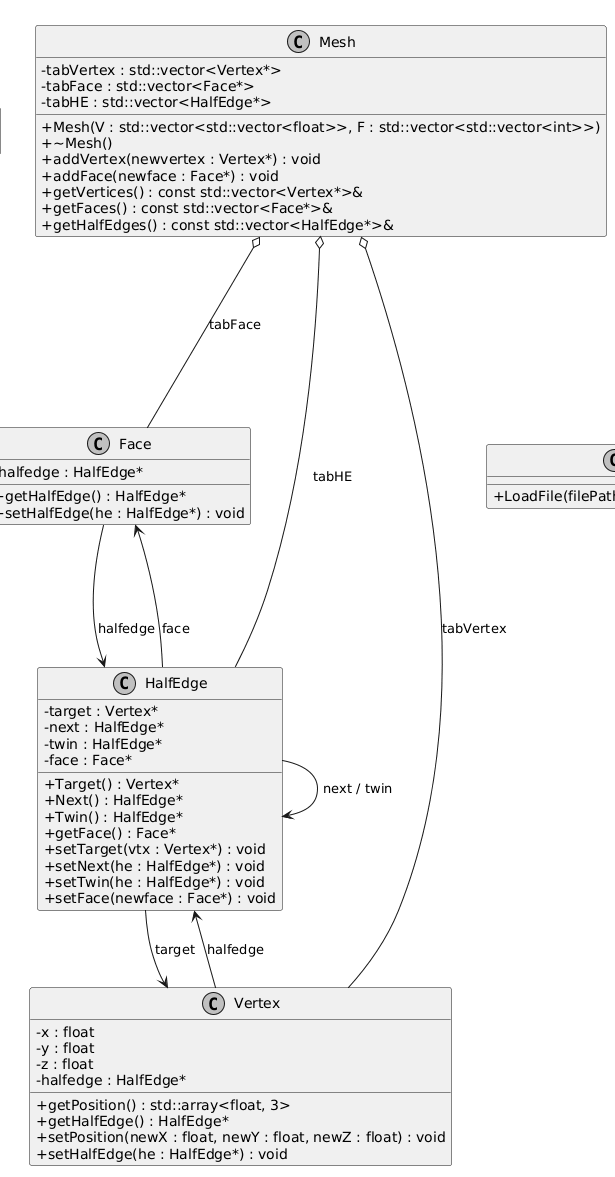
\includegraphics[width=0.55\textwidth]{mesh.png}
    \caption{Diagramme UML de la structure Mesh}
    \label{fig:uml_mesh}
\end{figure}

Dans cette partie, nous voyons le diagramme UML de la structure du Mesh, qui représente un maillage 3D. La classe \texttt{Mesh} contient des attributs pour stocker les sommets, les faces et les arêtes du maillage, ainsi que des méthodes pour gérer ces éléments. Les relations entre les classes sont également représentées, montrant comment elles interagissent pour former la structure globale du projet.

\begin{figure}[H]
    \centering
    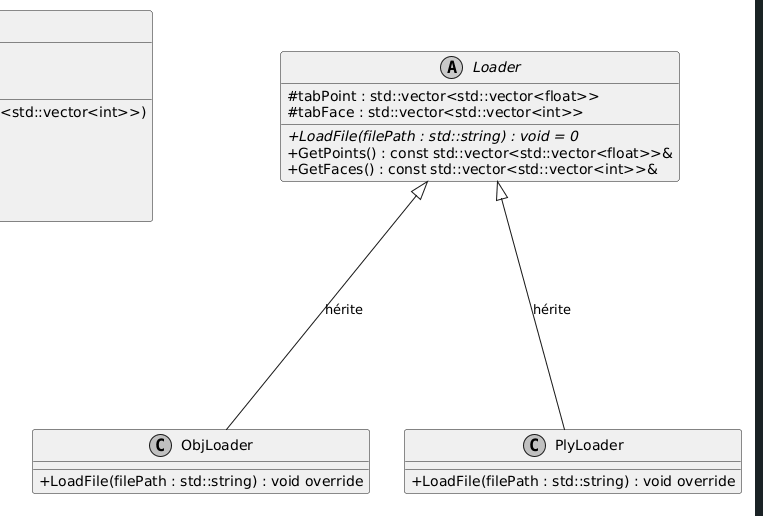
\includegraphics[width=0.55\textwidth]{loader.png}
    \caption{Diagramme UML du Loader}
    \label{fig:uml_loader}
\end{figure}

Pour le loader, nous avons utilisé une classe générique pour permettre le chargement de différents formats de fichiers. 
Grâce à cela, nous avons pu créer des classes spécifiques pour chaque format de fichier, telles que \texttt{PLYLoader} et \texttt{OBJLoader}, qui héritent de la classe générique \texttt{Loader}. Cela nous a permis de gérer facilement l'ajout de nouveaux formats de fichiers à l'avenir.

\newpage
\section{Loader}

Le système de chargement des fichiers de notre projet repose actuellement sur deux classes spécifiques, \texttt{PlyLoader} et \texttt{ObjLoader}, qui héritent toutes deux de la classe générique \texttt{Loader}.

La classe \texttt{PlyLoader} permet de charger les fichiers au format \texttt{.ply}, qu'ils soient encodés en ASCII ou en binaire au format \textit{Little Endian}. Elle commence par lire l'en-tête du fichier afin d'en déterminer le format, le nombre de sommets, le nombre de faces, les types de données utilisés (\texttt{double}, \texttt{float}, \texttt{int}), ainsi que la présence éventuelle de propriétés supplémentaires, telles que la couleur ou l'opacité. 
L'implémentation de ce chargeur a notamment nécessité la gestion des octets à ignorer lors de la lecture des données binaires, par exemple ceux correspondant au remplissage (\textit{padding}) ou à des propriétés qui ne sont pas exploitées par le programme. Nous avons utilisé des outils d'intelligence artificielle pour nous aider à mettre en œuvre cette gestion et à découvrir des outils C++ adaptés, comme \texttt{std::istringstream}, qui facilite l'analyse des données au format ASCII.

La classe \texttt{ObjLoader} permet de charger les fichiers au format \texttt{.obj}. Elle analyse chaque ligne du fichier en fonction de son préfixe afin de distinguer les sommets, identifiés par \texttt{v}, des faces, identifiées par \texttt{f}. L'utilisation de \texttt{std::istringstream} permet de séparer et d'extraire facilement les différentes valeurs présentes sur chaque ligne.

Enfin, les deux classes stockent les données extraites dans deux tableaux : \texttt{tabPoint} et \texttt{tabFace}. Le premier contient les coordonnées des sommets sous la forme d'un \texttt{std::vector<Eigen::Vector3d>}, tandis que le second contient les faces sous la forme d'un \texttt{std::vector<std::vector<int>>}. Cette organisation permet de représenter les sommets et la connectivité du modèle 3D dans des structures de données directement exploitables par le reste du programme.

\newpage
\section{Halfedge}

Notre structure Halfedge repose sur trois classes étroitement liées : \texttt{Vertex}, \texttt{Face} et \texttt{HalfEdge}.

La classe \texttt{Vertex} représente les sommets du maillage. Chaque sommet possède notamment une position, stockée sous la forme d'un \texttt{Eigen::Vector3d}, ainsi qu'un pointeur vers un objet \texttt{HalfEdge*} qui lui est associé.

La classe \texttt{Face} représente les faces triangulaires du maillage. Elle contient un pointeur vers l'un des objets \texttt{HalfEdge} qui la constituent, de type \texttt{HalfEdge*}. Les autres objets \texttt{HalfEdge} de la face peuvent ensuite être retrouvés en parcourant les liens entre eux.

La classe \texttt{HalfEdge} constitue le cœur de cette structure de données. Chaque objet \texttt{HalfEdge} contient plusieurs informations permettant de décrire sa position dans le maillage : un pointeur vers le sommet cible (\textit{target}), de type \texttt{Vertex*}, un pointeur vers l'object \texttt{HalfEdge} suivant (\textit{next}), un pointeur vers son opposé (\textit{twin}), ainsi qu'un pointeur vers la face à laquelle il appartient (\texttt{Face*}).

L'organisation de ces liens permet de parcourir efficacement le maillage et d'accéder aux éléments voisins. Elle vise également à faciliter les opérations de modification de la géométrie et de la topologie du maillage. Cependant, ces fonctionnalités ne sont pas encore implémentées dans le projet.

La structure du maillage est générée par la classe \texttt{Mesh}, à partir des tableaux de sommets et de faces fournis par le module de chargement (\texttt{Loader}). Les éléments sont ensuite organisés dans trois tableaux : \texttt{tabVertex}, \texttt{tabFace} et \texttt{tabHE}, qui contiennent respectivement les sommets, les faces et les objets \texttt{HalfEdge} du maillage.

\newpage

\section{Affichage}

Pour l'affichage, nous avons utilisé la bibliothèque \texttt{OpenGL}, qui est une API graphique puissante et flexible pour le rendu 2D et 3D. OpenGL nous permet de créer des scènes 3D interactives et de gérer les transformations, l'éclairage et les textures.

Voici les sommets d'un cube que nous avons utilisé pour tester l'affichage dans notre éditeur 3D :
\begin{figure}[H]
    \centering
    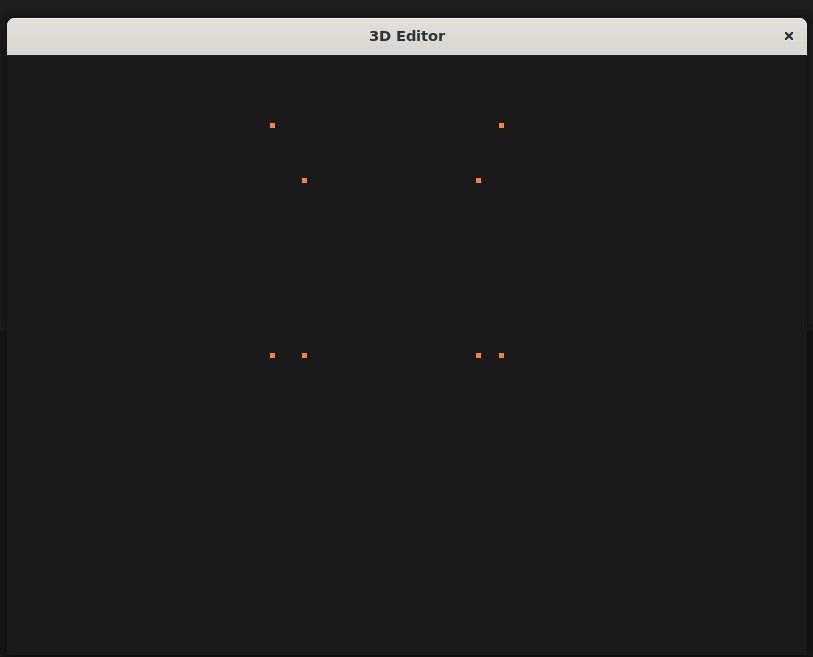
\includegraphics[width=0.5\textwidth]{point.jpeg}
    \caption{Sommets d'un cube pour le test d'affichage}
    \label{fig:cube}
\end{figure}

Ainsi que les faces triangulaires de ce dernier :
\begin{figure}[H]
    \centering
    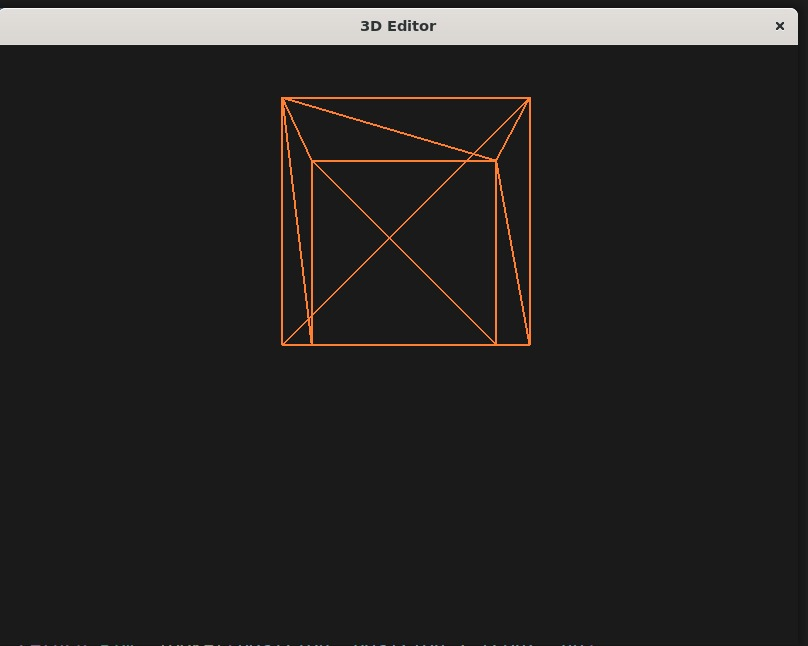
\includegraphics[width=0.5\textwidth]{ligne.jpeg}
    \caption{Faces triangulaires d'un cube pour le test d'affichage}
    \label{fig:cube_faces}
\end{figure} 

Par rapport au déplacement de la caméra, seuls les déplacements grâce aux touches ZQSD sont implémentés pour le moment. Le déplacement de la caméra est réalisé en modifiant la position de celle-ci dans l'espace 3D en fonction des entrées de l'utilisateur. Nous avons également prévu d'ajouter des fonctionnalités supplémentaires, telles que le zoom et la rotation de la caméra, pour améliorer l'expérience utilisateur.

\newpage

\section{Conclusion}

La majorité des bases structurelles du projet a été mise en place. Cependant, plusieurs fonctionnalités restent à développer afin d'atteindre les objectifs fixés. 

La principale difficulté rencontrée au cours du projet est notre manque d'expérience en C++, notamment dans l'utilisation d'OpenGL, ainsi que notre connaissance encore limitée des différentes fonctions proposées par les bibliothèques que nous utilisons. Cela nous a demandé du temps pour comprendre leur fonctionnement et les utiliser correctement. 

Plusieurs fonctionnalités restent à implémenter pour la suite du projet, comme la modification de la géométrie du modèle chargé, le calcul du plus court chemin entre deux sommets quelconques, l'optimisation des performances du programme, ainsi qu'une meilleure gestion des erreurs et des éventuels plantages.

\end{document}